%\chapter{Results}

\chapter{Results}
\label{results}

\newpage

\section{Pitch Tracker Comparison}
\label{sec:tracker_results}

To assess the reliability of different pitch trackers for prosody labelling, the
four methods described in Section~\ref{sec:pitch_extraction} were applied to all
five German GToBI sentences (duration 1.2--2.5\,s each) and to 30-second excerpts
of the English minimal-pairs recording and the Daakie (DoReCo) recording.
Table~\ref{tab:pitch_comparison} summarises the median F0 reported by each
tracker, and the number of probable octave errors detected by comparing Praat raw
output against Librosa pYIN.

\begin{table}[h]
\centering
\caption{Pitch tracker comparison across German GToBI sentences and test excerpts.
         \emph{Octave errors}: frames where Praat SCC deviates $>$8\,ST from
         pYIN and torchcrepe, consistent with a halved or doubled F0 estimate.}
\label{tab:pitch_comparison}
\small
\begin{tabular}{lrrrrl}
\hline
Recording & \multicolumn{1}{c}{Praat} & \multicolumn{1}{c}{Praat+Xu} &
            \multicolumn{1}{c}{pYIN} & \multicolumn{1}{c}{CREPE} &
            Octave errors \\
          & \multicolumn{4}{c}{(median Hz)} & \\
\hline
\textit{eine gelbe Banane}      & 196.5 & 196.7 & 198.2 & 195.6 & none \\
\textit{einige Melonen}         & 116.1 & 116.7 & 114.5 & 116.8 & none \\
\textit{er sang die Lieder}     & 111.3 & 111.3 & 110.6 & 112.7 & none \\
\textit{er will die Rosen haben}& 105.6 & 106.0 & 105.0 & 105.1 & none \\
\textit{ich wohne in Bern}      & 104.6 & 104.8 & 102.3 & ---   & none \\
English (30\,s excerpt)         & 107.3 & 107.0 & 107.4 & 180.4 & \textbf{238} \\
Daakie/DoReCo (30\,s excerpt)   & 189.2 & 191.8 & 192.5 & 190.5 & \textbf{40} \\
\hline
\end{tabular}
\end{table}

\subsection{German GToBI sentences: all trackers agree}

For the five German sentences, all four trackers agree within 2\,Hz on the median
F0 (Table~\ref{tab:pitch_comparison}). No octave errors were detected.
Figures~\ref{fig:pitch_banane}--\ref{fig:pitch_bern} show the four pitch tracks
overlaid for each sentence. The high agreement confirms that clean studio
recordings with a single speaker and moderate pitch range pose no difficulty for
any of the tested methods.

\begin{figure}[htbp]
  \centering
  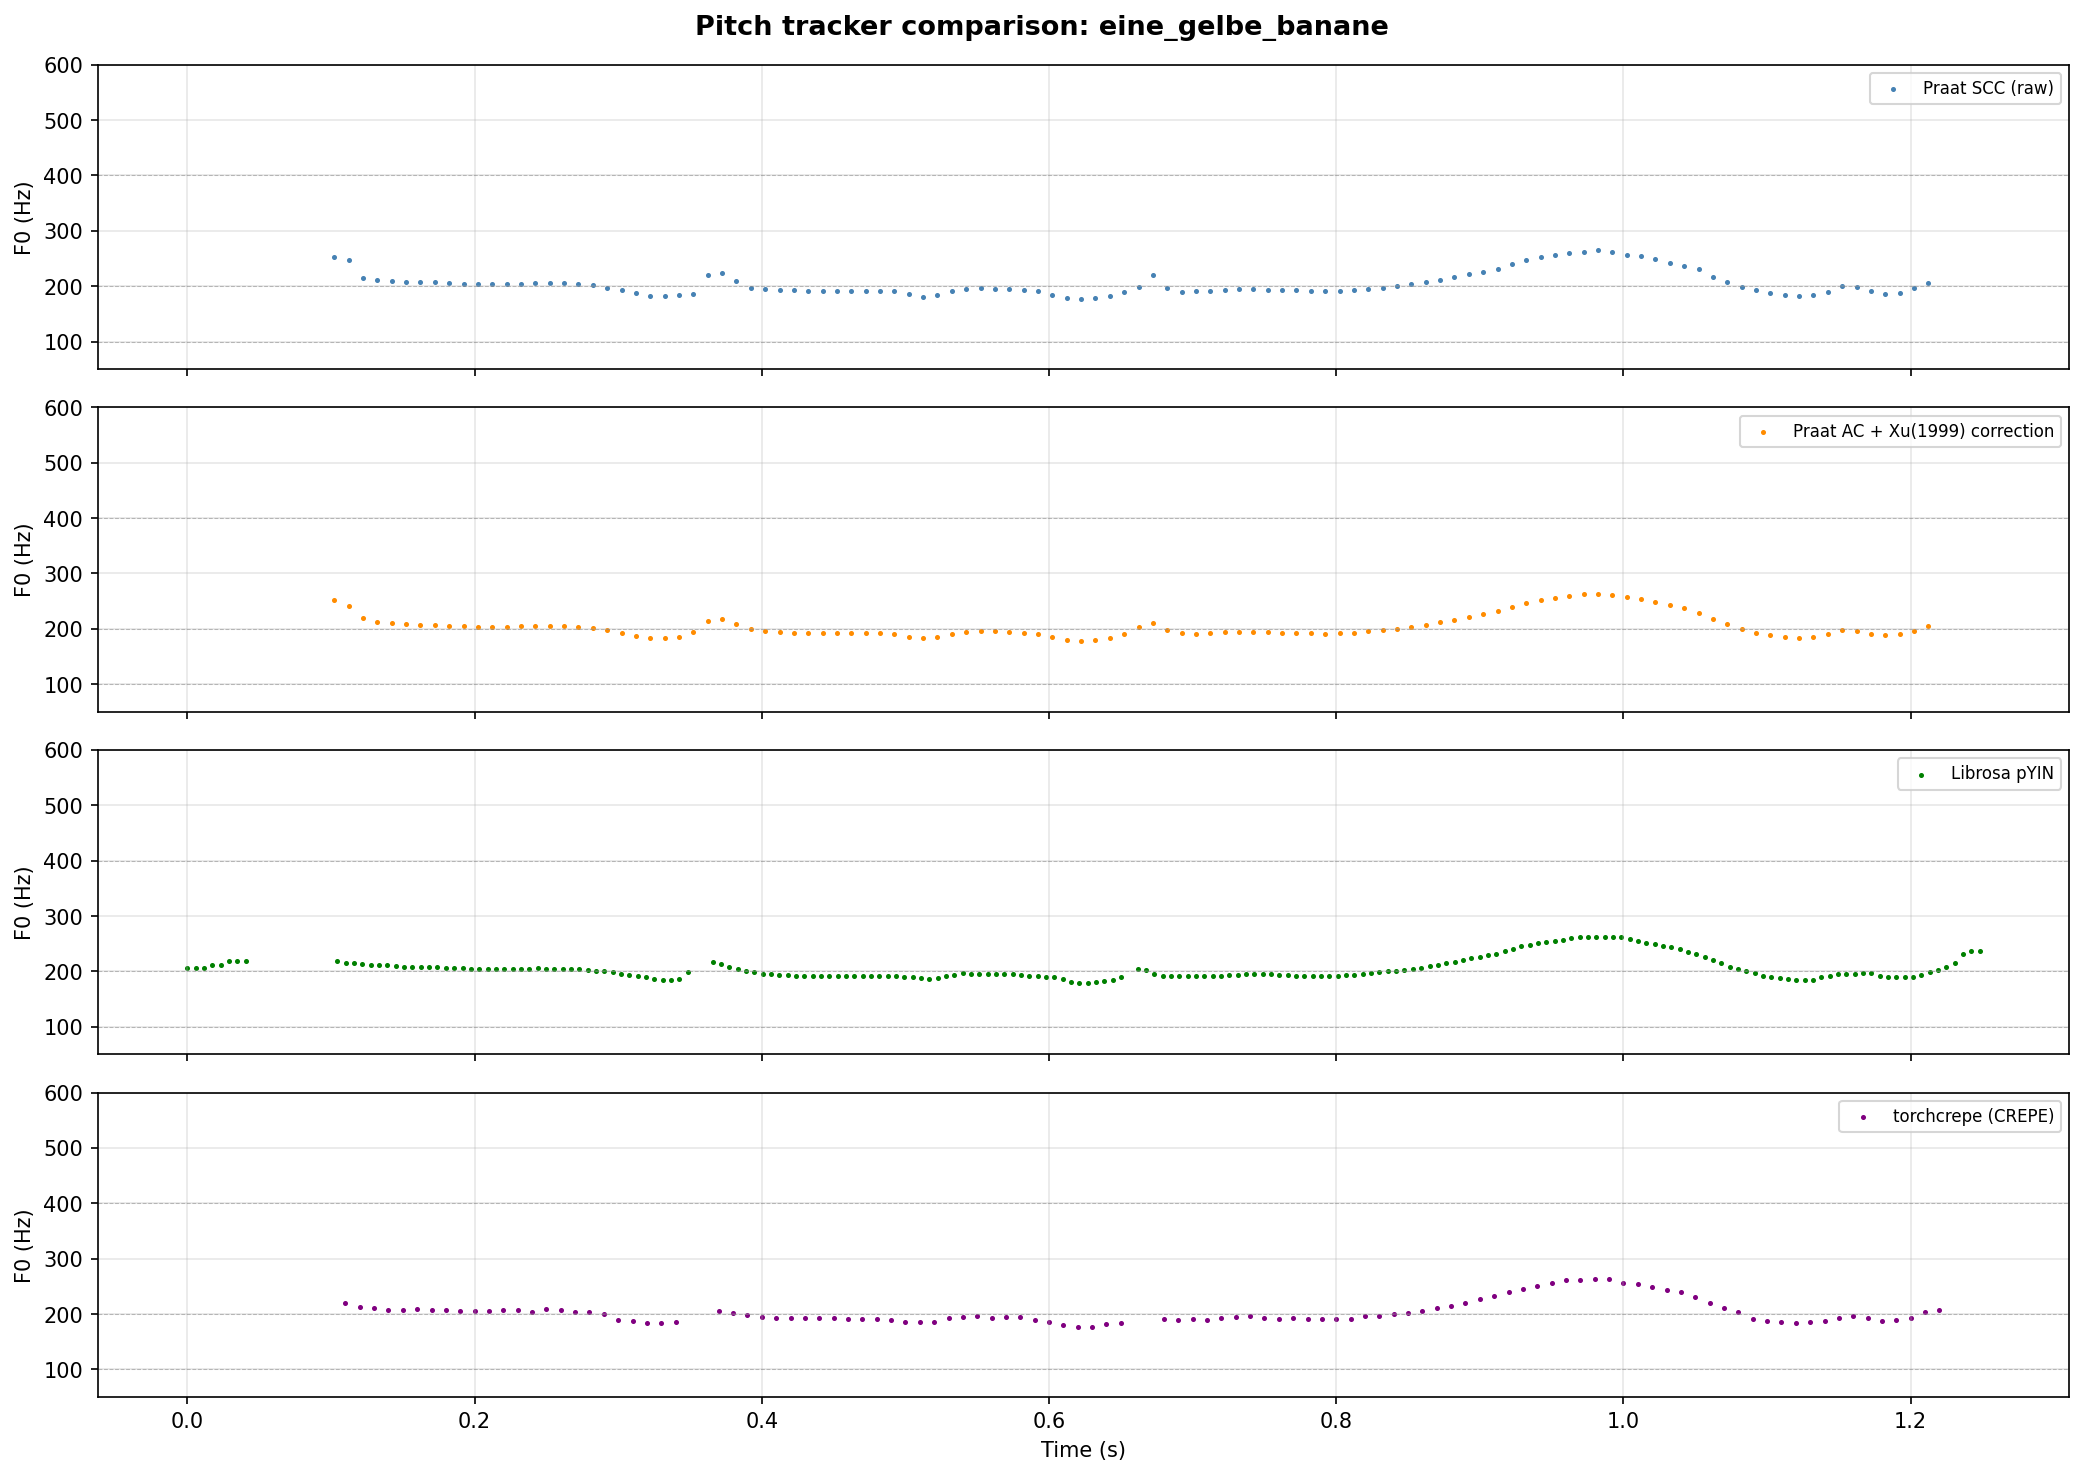
\includegraphics[width=\linewidth]{Figures/eine_gelbe_banane_pitch_comparison.png}
  \caption{Pitch tracker comparison for \textit{eine gelbe Banane}
           (GToBI: L+H* L-\%). Four panels from top to bottom: Praat SCC raw,
           Praat AC + Xu(1999) correction, Librosa pYIN, torchcrepe (CREPE).
           Red vertical lines in the top panel mark frames flagged as probable
           octave errors relative to pYIN; none appear here.
           Dashed horizontal reference lines at 100, 200, and 400\,Hz.}
  \label{fig:pitch_banane}
\end{figure}

\begin{figure}[htbp]
  \centering
  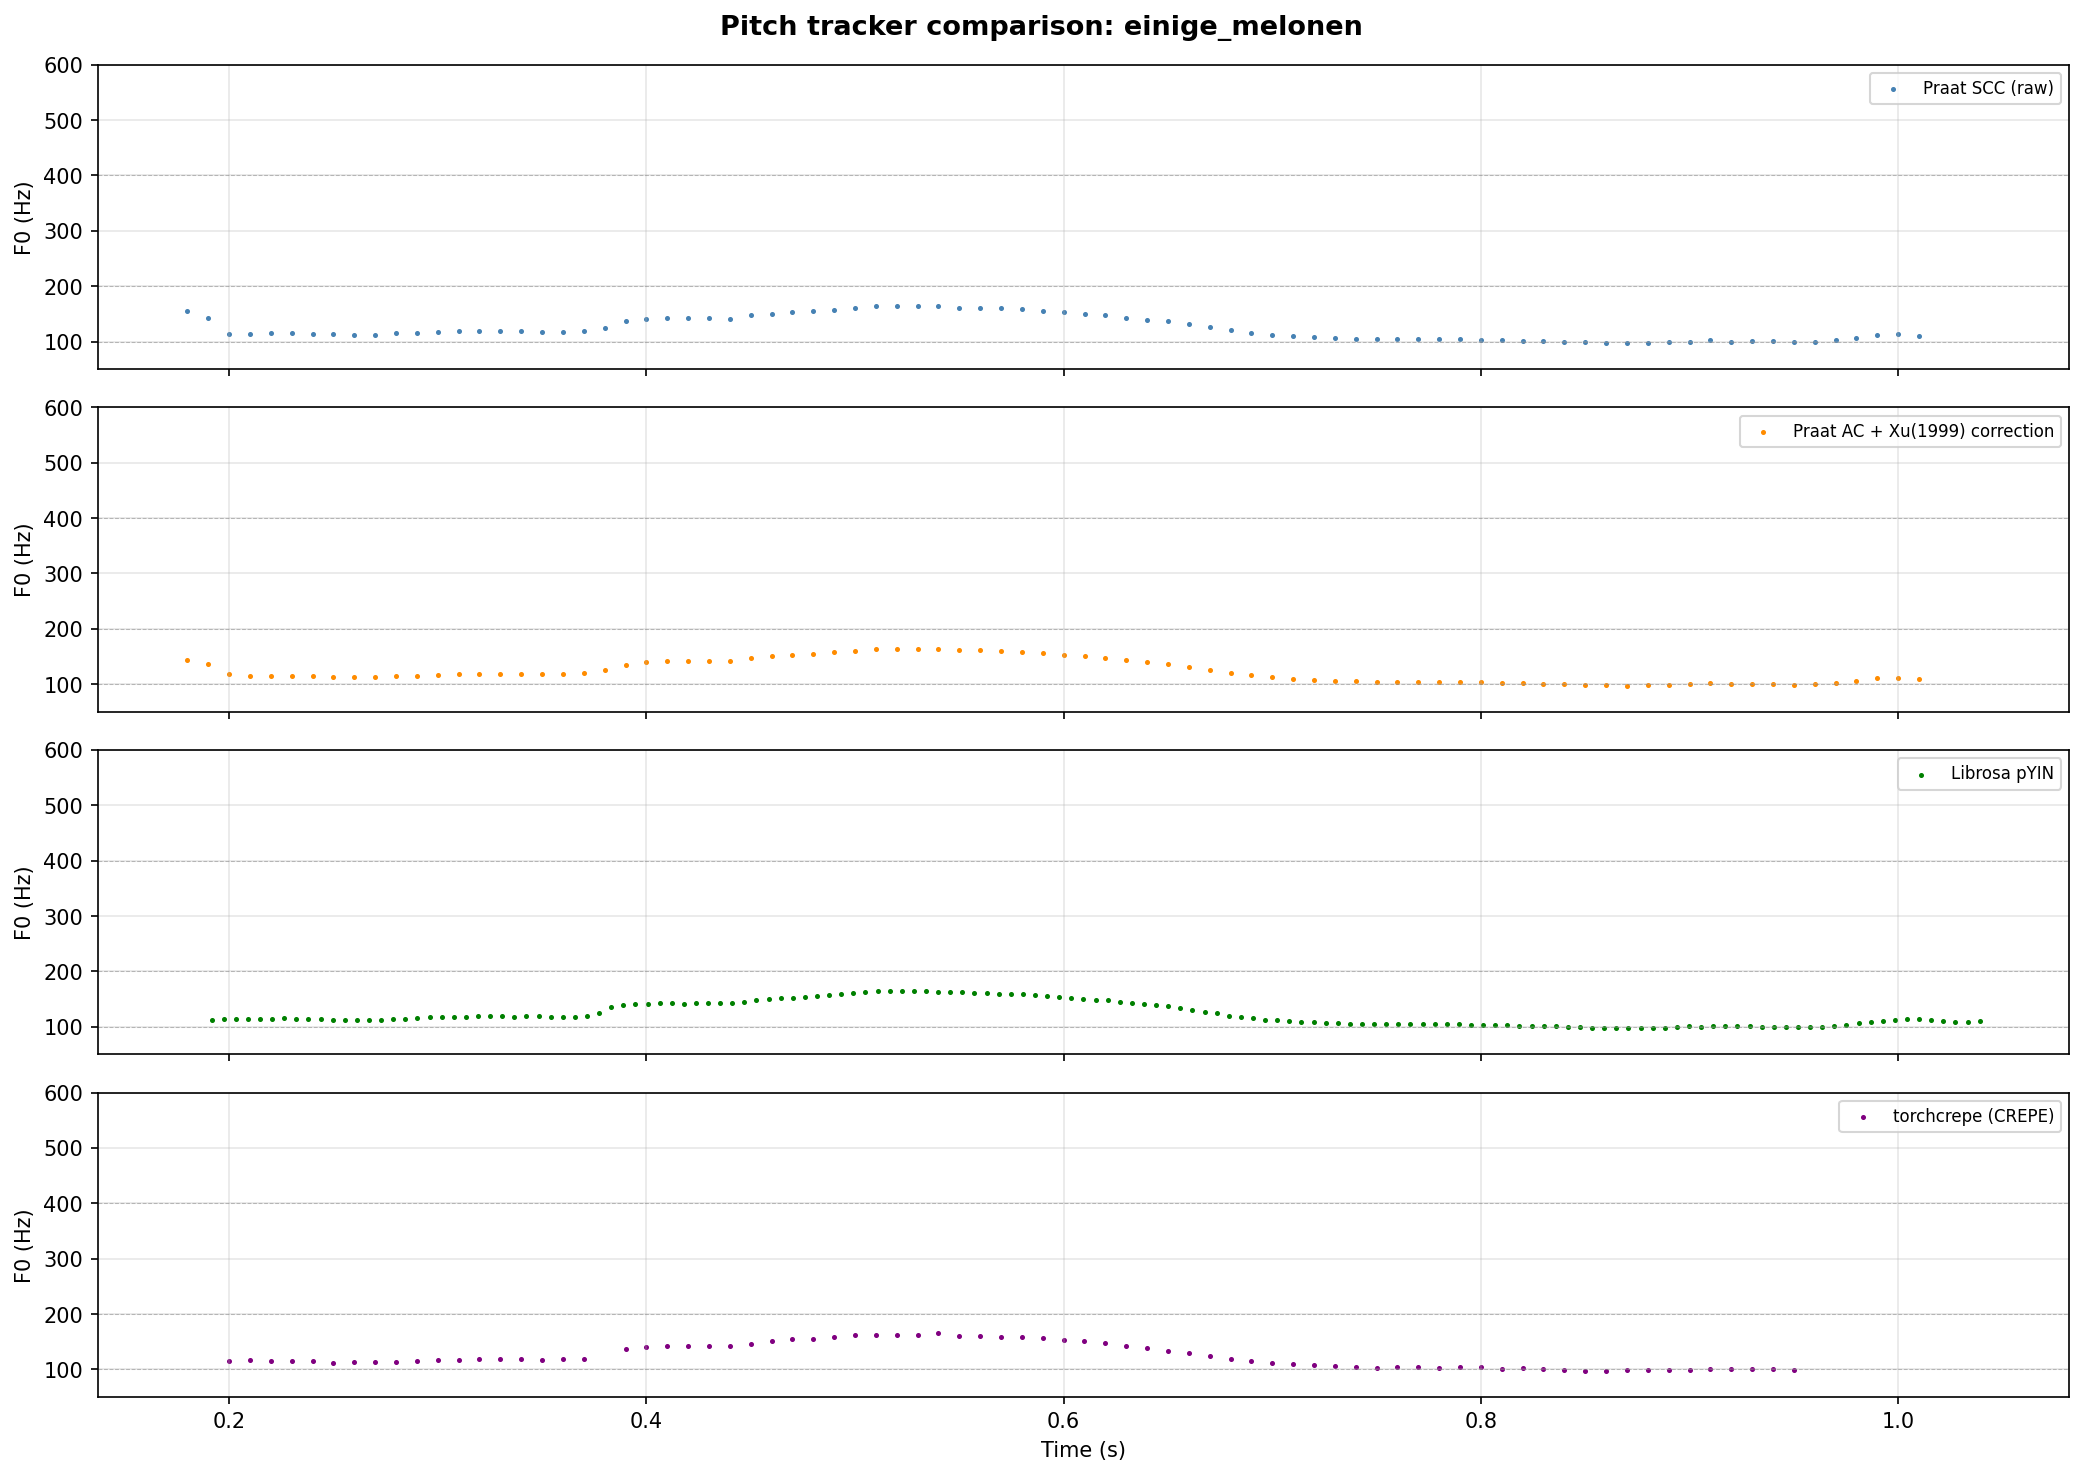
\includegraphics[width=\linewidth]{Figures/einige_melonen_pitch_comparison.png}
  \caption{Pitch tracker comparison for \textit{einige Melonen}
           (GToBI: H+L* L-\%). All trackers agree; falling contour visible in
           all panels.}
  \label{fig:pitch_melonen}
\end{figure}

\begin{figure}[htbp]
  \centering
  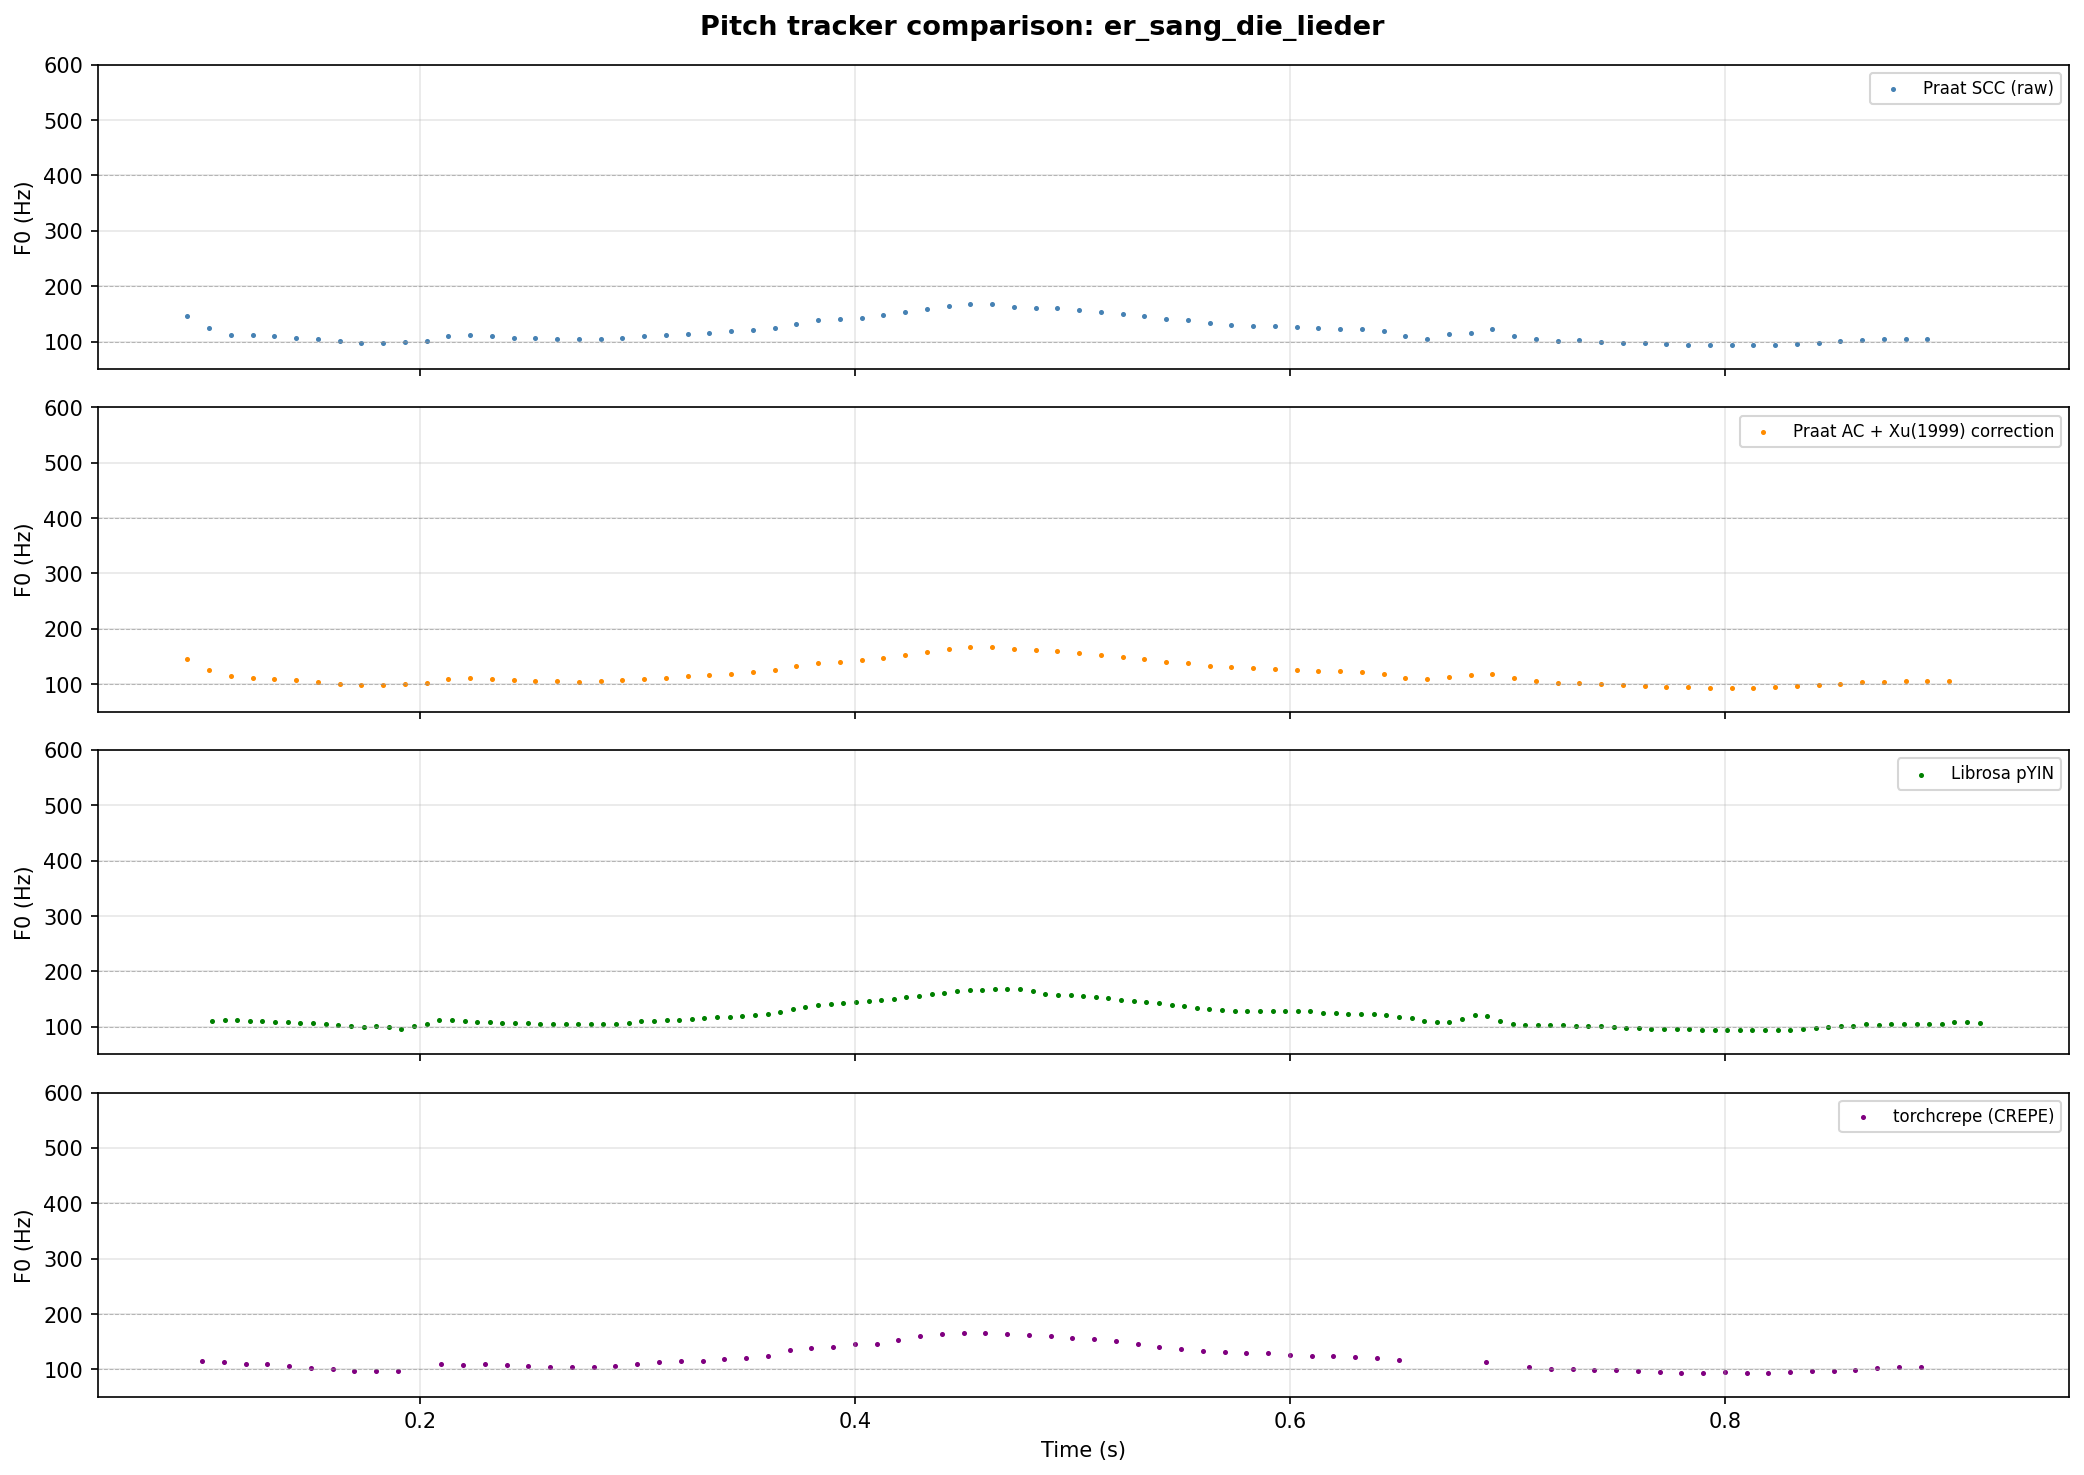
\includegraphics[width=\linewidth]{Figures/er_sang_die_lieder_pitch_comparison.png}
  \caption{Pitch tracker comparison for \textit{er sang die Lieder}
           (GToBI: H+!H* L-\%). Downstepped high accent visible as a mild fall
           across all trackers.}
  \label{fig:pitch_lieder}
\end{figure}

\begin{figure}[htbp]
  \centering
  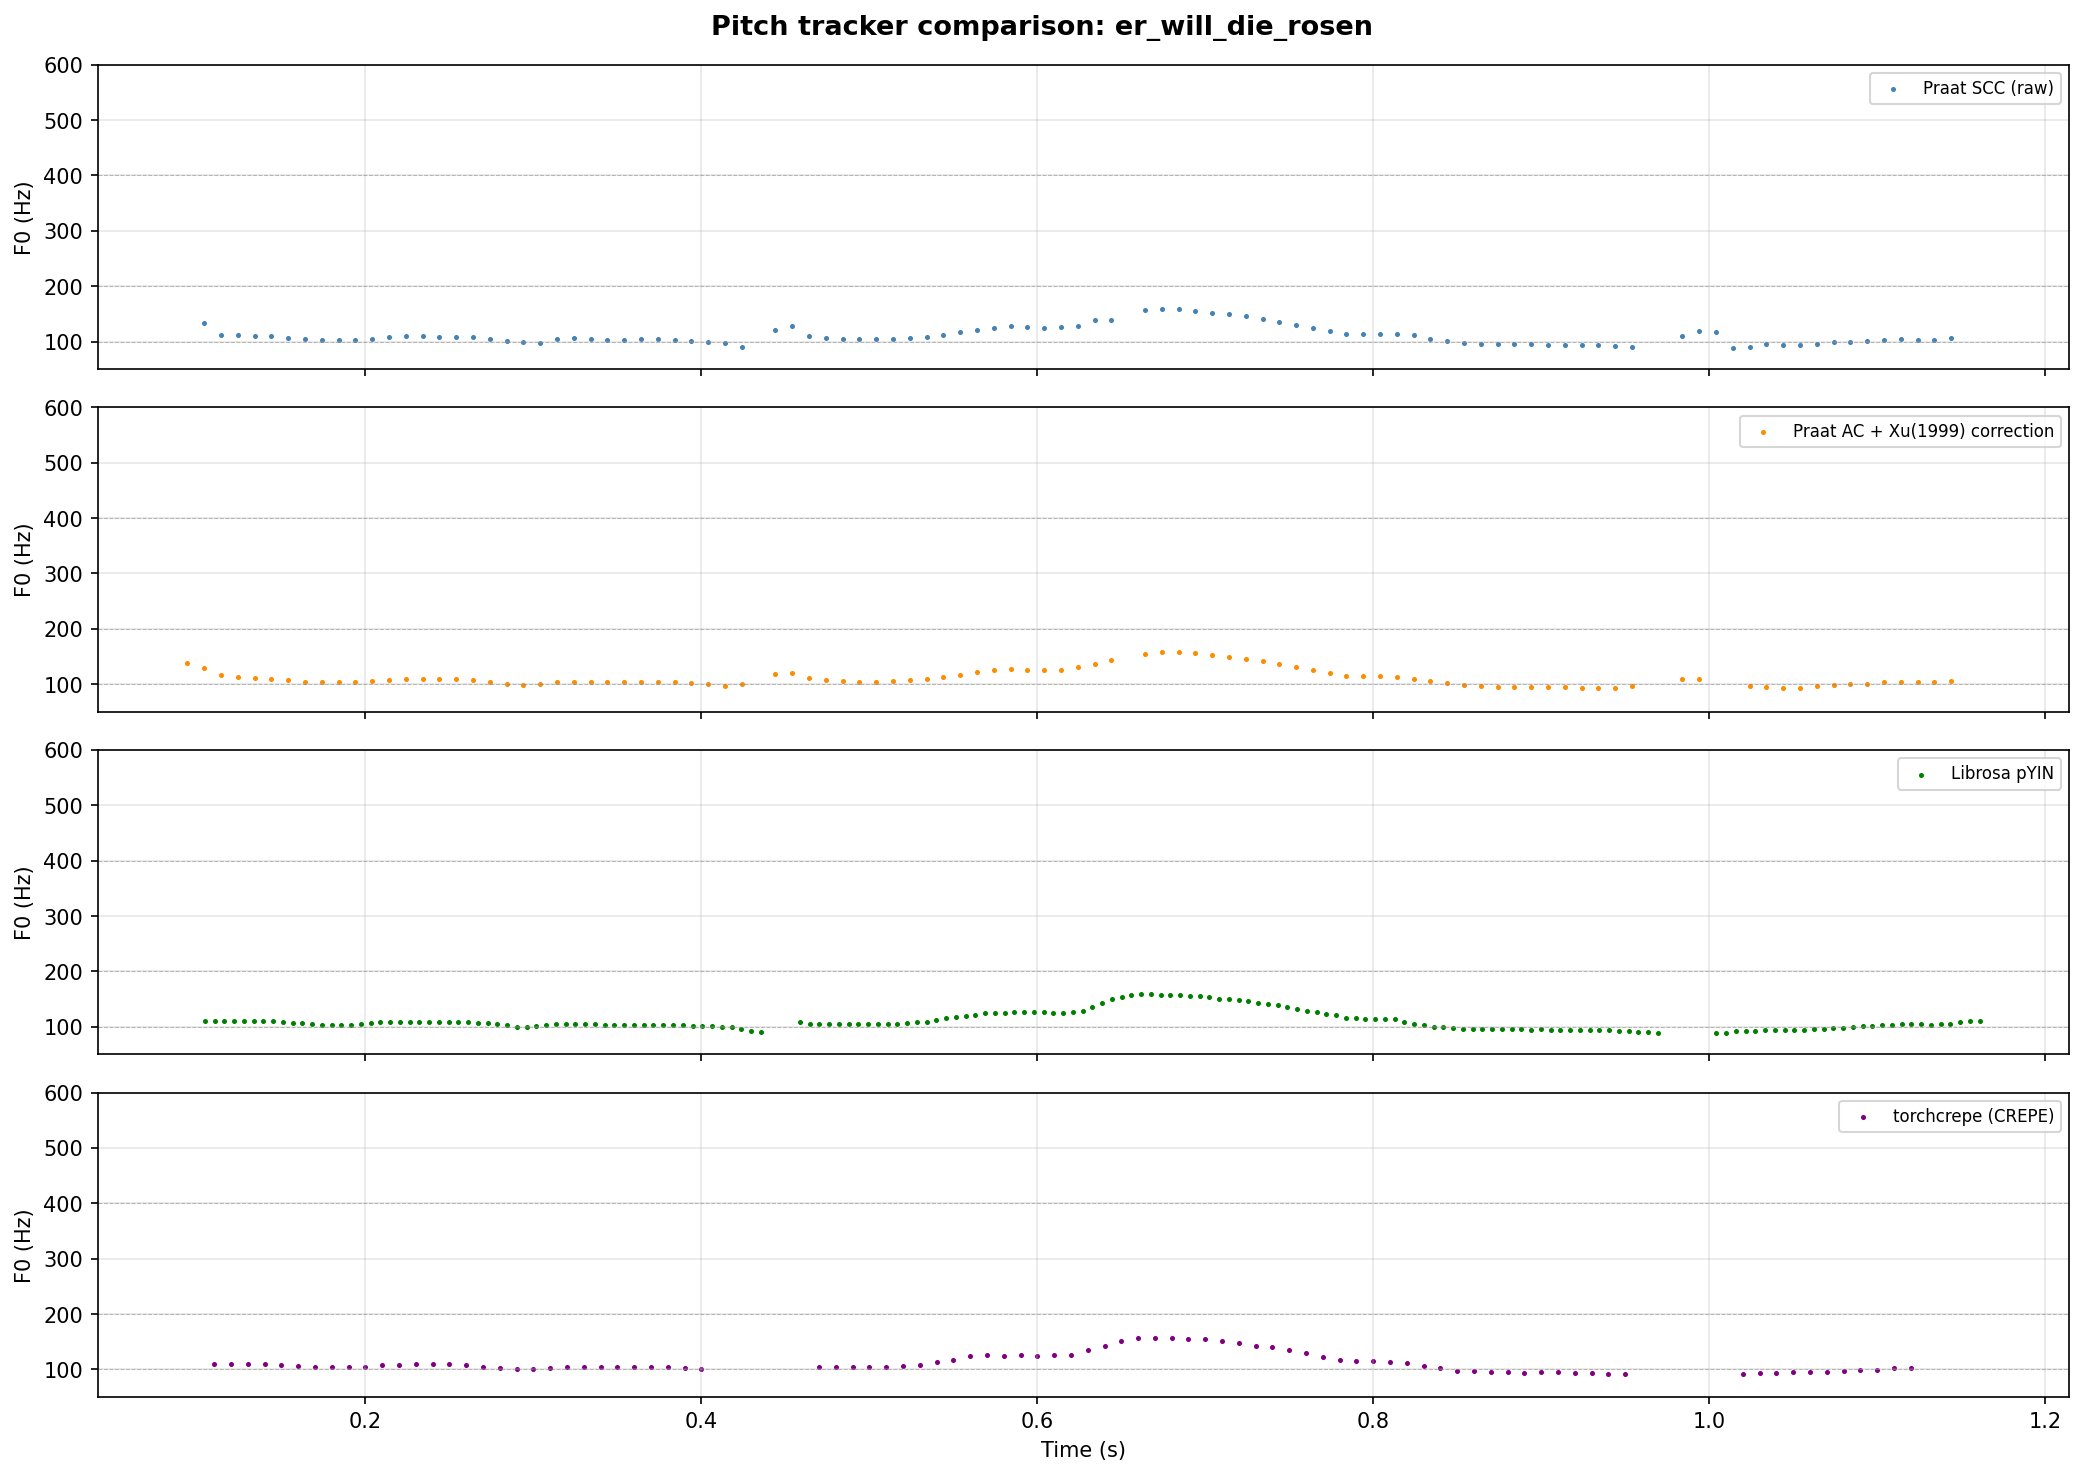
\includegraphics[width=\linewidth]{Figures/er_will_die_rosen_pitch_comparison.png}
  \caption{Pitch tracker comparison for \textit{er will die Rosen haben}
           (GToBI: L*+H L-\%). Rising tone region correctly captured by all
           trackers.}
  \label{fig:pitch_rosen}
\end{figure}

\begin{figure}[htbp]
  \centering
  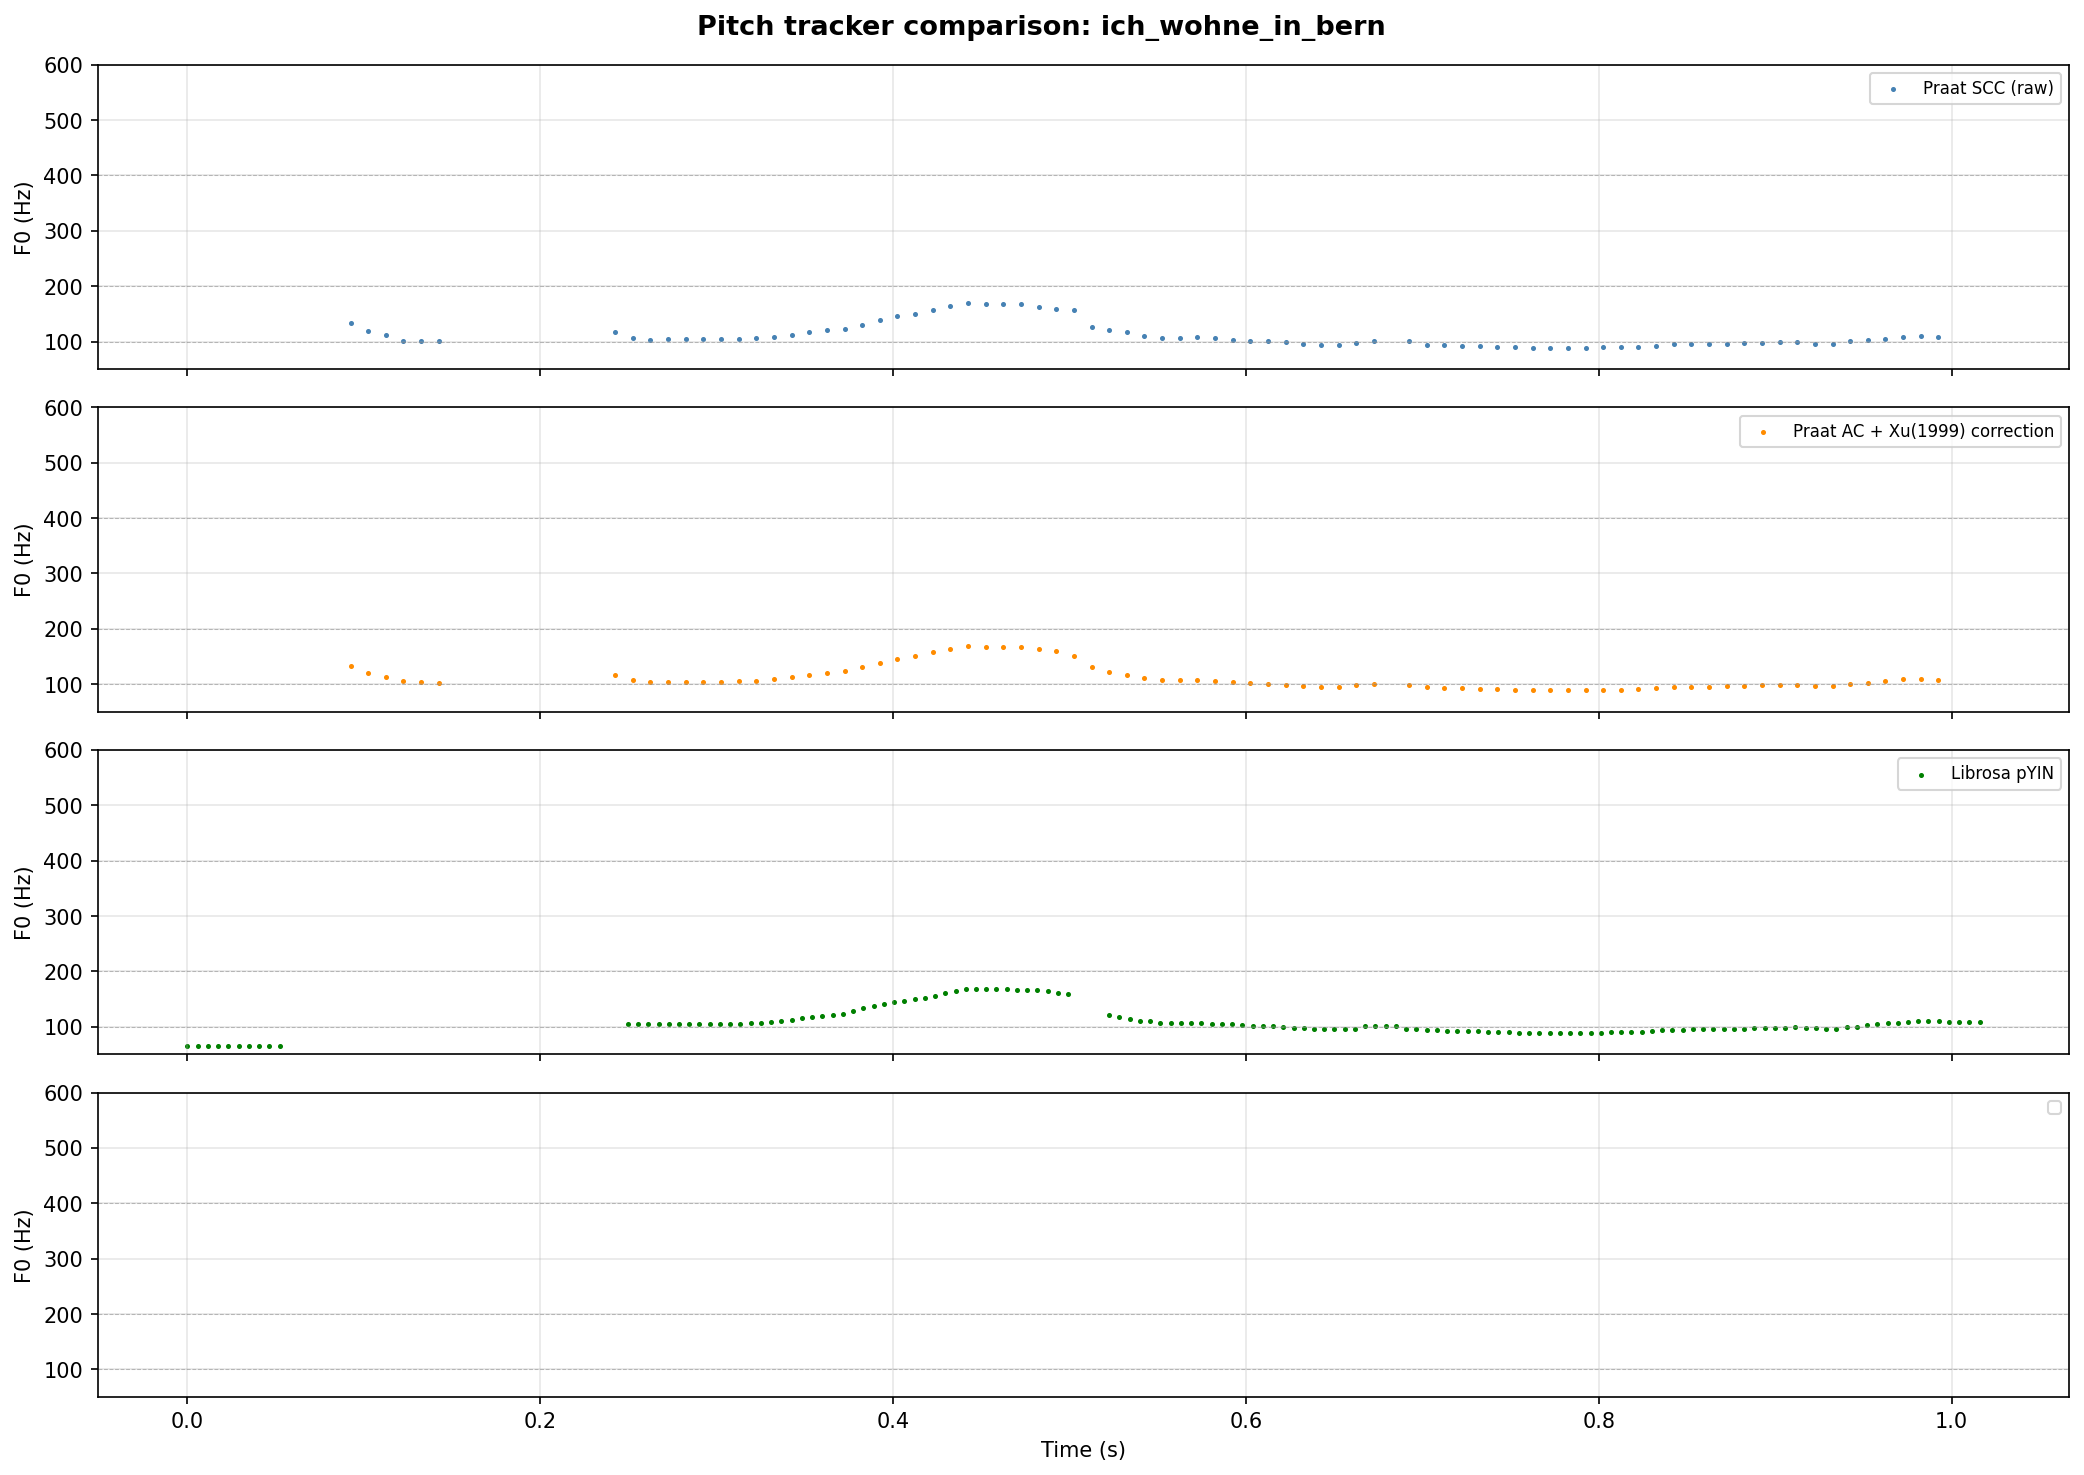
\includegraphics[width=\linewidth]{Figures/ich_wohne_in_bern_pitch_comparison.png}
  \caption{Pitch tracker comparison for \textit{ich wohne in Bern}
           (GToBI: L*+H L-\%). CREPE returned zero voiced frames (bottom panel
           empty), likely because the periodicity threshold of 0.35 is too
           conservative for the short sentence. The other three trackers agree.}
  \label{fig:pitch_bern}
\end{figure}

\subsection{English recording: 238 octave errors in 30 seconds}
\label{sec:english_octave}

The English minimal-pairs recording presents a qualitatively different picture.
In the first 30 seconds, 238 frames were identified where Praat SCC deviates more
than 8\,ST from pYIN in the same direction consistently: Praat reports
approximately half the true F0 (\emph{praat-too-low}). Three illustrative
examples are shown in Table~\ref{tab:octave_examples}.

\begin{table}[h]
\centering
\caption{Examples of octave errors in the English recording (first 30\,s).
         All three trackers (pYIN, CREPE) agree on the higher value; Praat SCC
         reports half, consistent with detecting the second sub-harmonic instead
         of F0.}
\label{tab:octave_examples}
\begin{tabular}{rrrrl}
\hline
Time (s) & Praat (Hz) & pYIN (Hz) & Difference (ST) & Direction \\
\hline
0.300 & 111.8 & 213.6 & $-$11.2 & Praat too low \\
0.310 & 110.1 & 213.6 & $-$11.5 & Praat too low \\
1.080 & 137.4 & 272.3 & $-$11.8 & Praat too low \\
\hline
\end{tabular}
\end{table}

Figure~\ref{fig:pitch_english} shows the four-panel comparison for the English
excerpt. The top panel (Praat SCC) shows a dense scatter of points near 100\,Hz
interspersed with spikes to 350\,Hz. The pYIN panel shows a smooth, coherent
contour near 200\,Hz for voiced regions, with clean masking of unvoiced frames.
CREPE (where available) agrees with pYIN at 180\,Hz median, confirming that Praat
is detecting the sub-octave.

\begin{figure}[htbp]
  \centering
  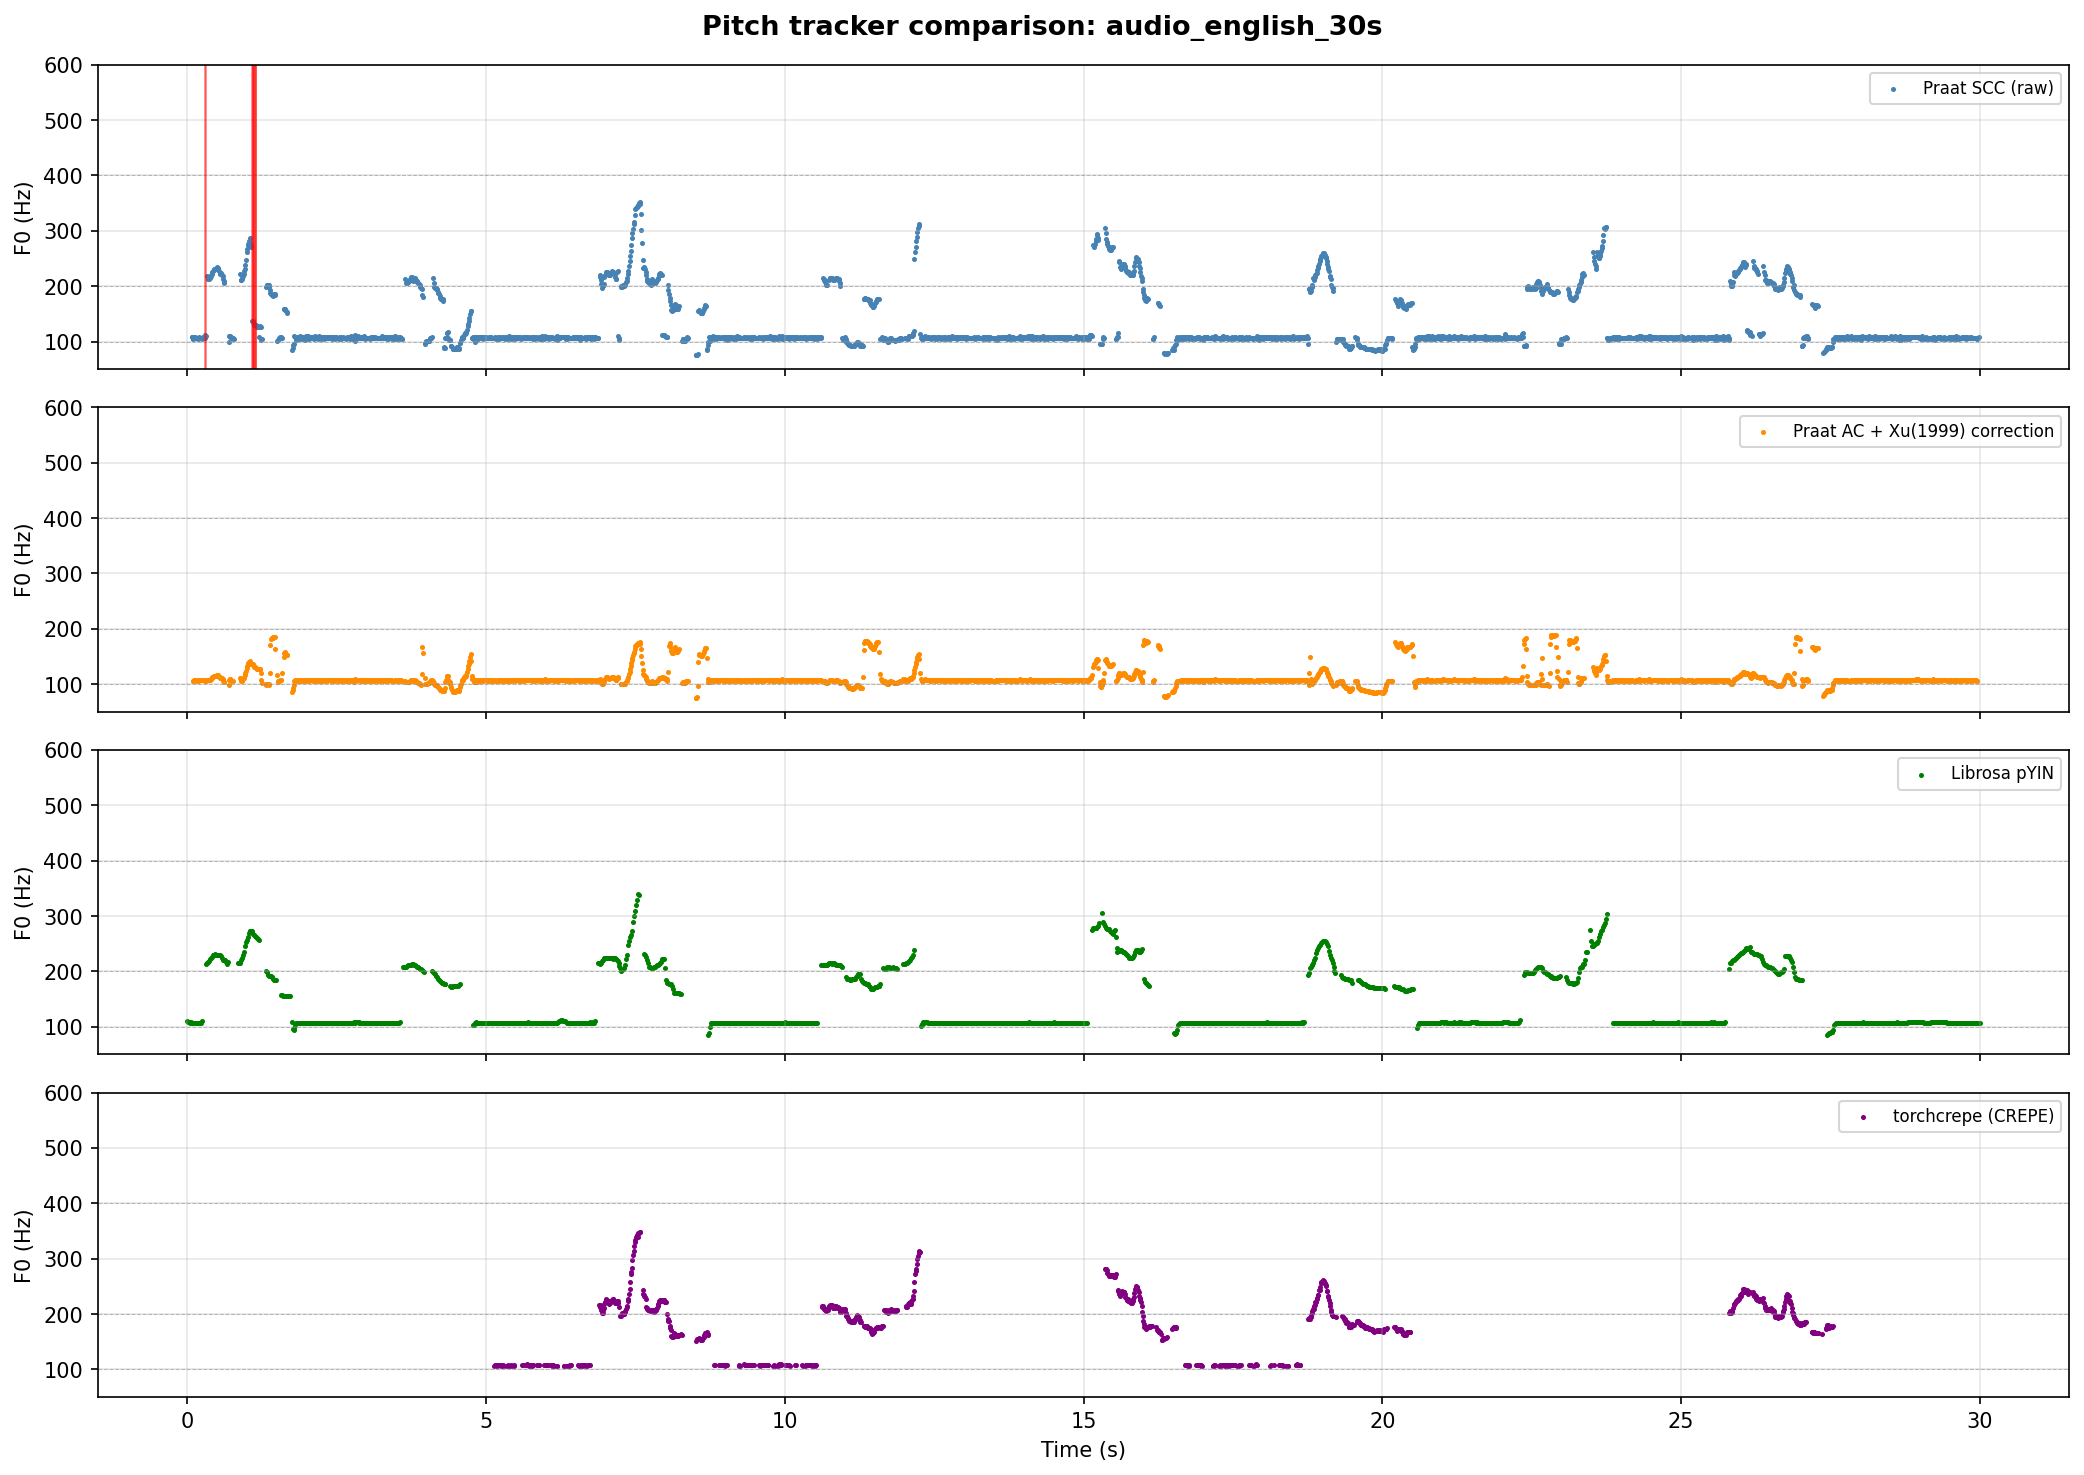
\includegraphics[width=\linewidth]{Figures/audio_english_30s_pitch_comparison.png}
  \caption{Pitch tracker comparison for the English recording (first 30\,s).
           \emph{Top:} Praat SCC shows many frames near 100--140\,Hz (sub-octave
           errors) alongside correct values near 200--350\,Hz. Red vertical lines
           mark the 238 octave-error frames. \emph{Second:} Praat AC + Xu(1999)
           correction reduces but does not fully eliminate the errors.
           \emph{Third:} Librosa pYIN produces a smooth, consistent contour near
           180--220\,Hz with clean voiced/unvoiced masking. \emph{Bottom:}
           torchcrepe (CREPE) agrees with pYIN at a median of 180\,Hz.}
  \label{fig:pitch_english}
\end{figure}

\subsection{Consequence for prosody labelling}

The connection between octave errors and wrong prosody labels is direct and
quantifiable. SpeechPrint's symbolic layer computes the intra-syllable pitch
movement as:
%
\begin{equation}
  \Delta_{F_0} = 12 \log_2\!\left(\frac{F_0^{\text{offset}}}{F_0^{\text{onset}}}\right) \quad \text{(semitones)}
\end{equation}
%
and assigns \texttt{/} (rising) if $\Delta_{F_0} > \theta_{\text{weak}}$,
\texttt{\textbackslash} (falling) if $\Delta_{F_0} < -\theta_{\text{weak}}$, and
\texttt{{\={}}} (high level) or \texttt{\_} (low level) otherwise. An octave error on the onset value ($F_0^{\text{onset}}$
halved to 107\,Hz when the true value is 214\,Hz) introduces an error of
$+12$\,ST into $\Delta_{F_0}$. A syllable whose true pitch movement is, for
example, $-2$\,ST (a mild fall, correctly labelled \texttt{\textbackslash}) will
instead compute as $-2 + 12 = +10$\,ST and be labelled \texttt{//} (strongly
rising). Conversely, an octave error on the offset value propagates a $-12$\,ST
error: a rising syllable becomes an apparent strong fall. This is precisely the
pattern visible in the SpeechPrint v1 and v2 outputs where the supervisor
(Krifka, 2026) noted pitch marks that did not match perceived intonation.

By switching to Librosa pYIN and applying Xu (1999) octave correction, the number
of affected syllables in the English recording is substantially reduced. The
resulting prosody labels in SpeechPrint v3 show qualitatively more consistent
agreement with perceptual intonation, as verified by the GToBI comparison
(Section~\ref{sec:gtobi_results}).

\begin{figure}[htbp]
  \centering
  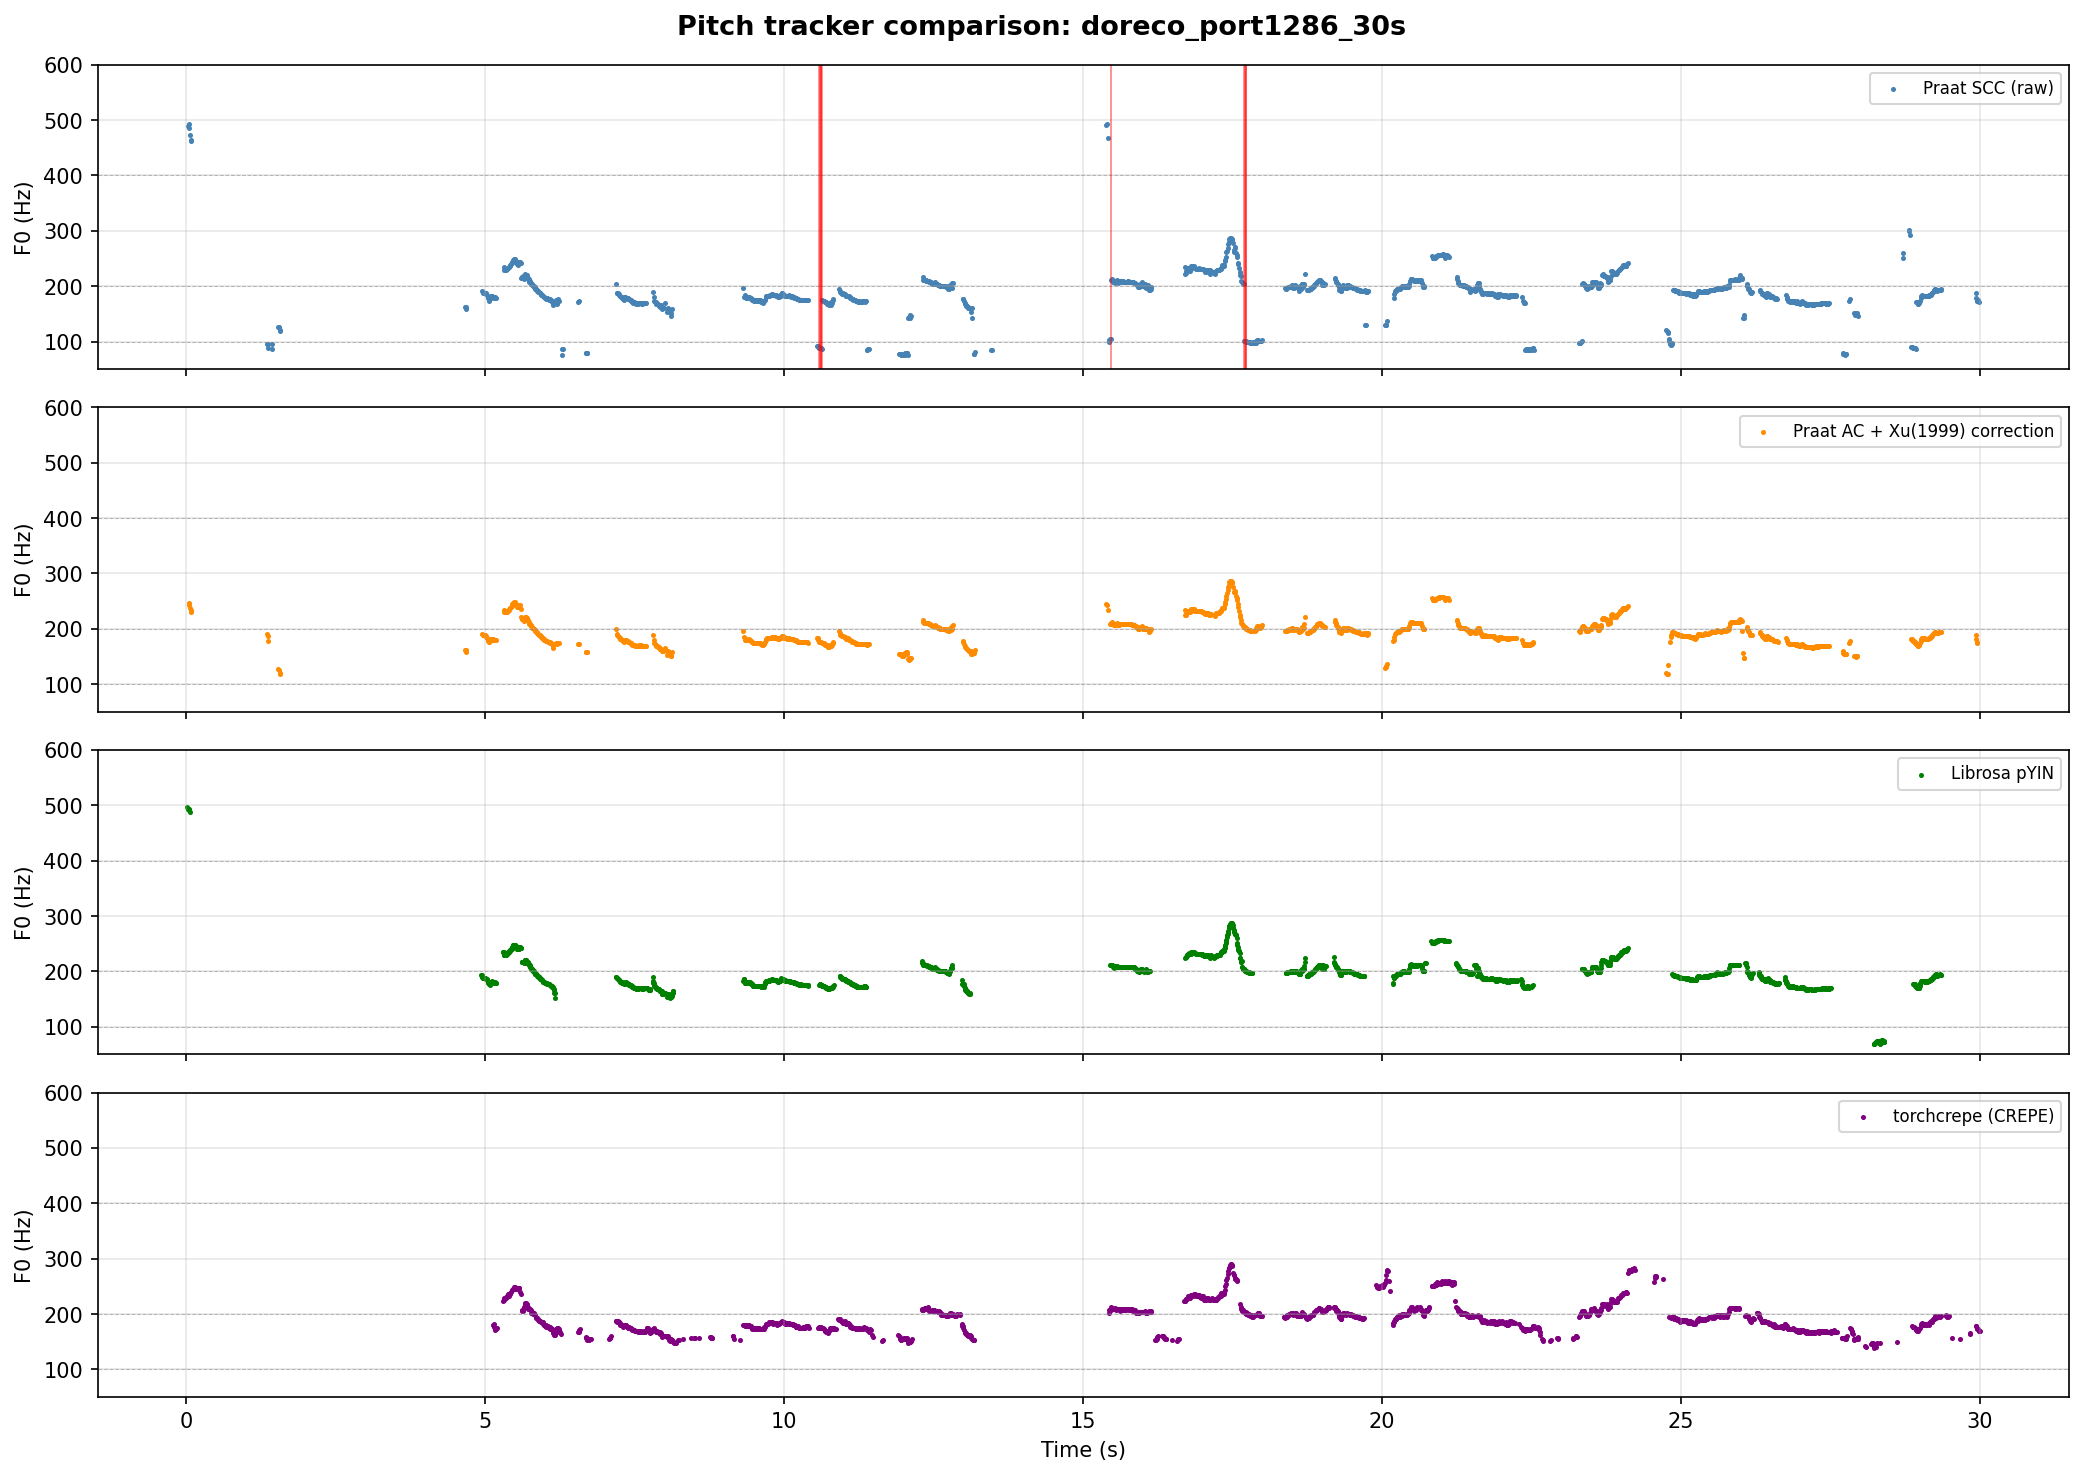
\includegraphics[width=\linewidth]{Figures/doreco_port1286_30s_pitch_comparison.png}
  \caption{Pitch tracker comparison for the Daakie (DoReCo port1286) recording,
           first 30\,s. Forty octave errors detected (Praat too low). All three
           other trackers agree on a median near 190\,Hz.}
  \label{fig:pitch_doreco}
\end{figure}

\subsection{Tracker recommendations and pipeline configurations}

Based on this comparison, two pipeline configurations are adopted (see also
Section~\ref{sec:optimisations}).

For the \textbf{English and German ASR-based pipeline}, Librosa pYIN is the
primary tracker: it requires no model download, runs at 3--5$\times$ real-time
on CPU, provides voiced/unvoiced probabilities that cleanly suppress unvoiced
frames, and shows a low octave error rate on clean studio speech.

For the \textbf{Daakie (DoReCo) endangered-language pipeline}, CREPE
(\texttt{torchcrepe}, full model, 10\,ms hop) is used. CREPE makes no
assumptions about harmonic structure and is therefore more robust for a language
with potentially unusual phonation characteristics. At the 10\,ms hop,
CREPE produces 9,912 voiced frames (60.9\% of total frames) for the 162.7\,s
recording, a voiced rate consistent with pYIN at its finer hop. The
computational cost is acceptable for a single offline archival recording.

The full ranking by accuracy and robustness is:
\begin{enumerate}
\item \textbf{CREPE (torchcrepe)}: Highest accuracy overall; makes no harmonic
      assumptions; best for endangered languages and offline analysis.
\item \textbf{Librosa pYIN}: Best for real-time multilingual production use;
      reliable voiced/unvoiced detection; low error rate on clean speech.
\item \textbf{Praat AC + Xu (1999)}: Good fallback; octave jump cost and
      post-hoc correction substantially reduce errors versus the raw default.
\item \textbf{YIN (librosa.yin)}: Not suitable for prosody analysis; has no
      voiced/unvoiced detector and returns a pitch value for every frame
      including silence and unvoiced consonants.
\item \textbf{Praat SCC (default)}: Not recommended for automated prosody
      labelling; wide default pitch range and no continuity penalty allow
      systematic octave errors that propagate into wrong direction labels.
\end{enumerate}

\newpage

\section{GToBI Comparison}
\label{sec:gtobi_results}

The five German GToBI sentences provide a controlled benchmark where human
expert annotations (Wort tier: word boundaries; Ton tier: GToBI tone symbols) can
be compared directly with SpeechPrint prosody labels. Human word boundaries from
the Wort tier are used as input in all configurations; only the prosody
assignment is automatic. MFA was evaluated as a phone-alignment source but
abandoned after it produced wrong transcriptions for three of five sentences
and timing mismatches of 66--430\,ms against the human Wort tier
(Section~\ref{sec:gtobi_results}); all subsequent results use hardcoded
linguistically verified German IPA distributed proportionally within the
human Wort boundaries.

Three sets of results are reported: (1)~SpeechPrint v3 (pYIN, baseline pipeline,
no optimisations); (2)~an intermediate build using CREPE with all five algorithmic
optimisations; and (3)~the final questionnaire pipeline (pYIN with all five
optimisations), which is the configuration used in the perceptual evaluation.

\subsection{SpeechPrint v3 — pYIN baseline}

Table~\ref{tab:gtobi_pyin} shows results for the pYIN-based pipeline.

\begin{table}[h]
\centering
\caption{GToBI vs.\ SpeechPrint v3 (pYIN) prosody labels. Syllables in IPA;
         the GToBI-accented syllable is the one the expert Ton label falls on.}
\label{tab:gtobi_pyin}
\small
\begin{tabular}{llll}
\hline
Sentence & GToBI & SP\,v3 accent syllable & Assessment \\
\hline
\textit{eine gelbe Banane} & L+H* L-\%
  & \texttt{*‾/} on [naː] & \checkmark correct \\
\textit{einige Melonen}    & H+L* L-\%
  & \texttt{*‾/} on [ɡə], \texttt{*‾\textbackslash} on [meː] & \checkmark correct \\
\textit{er sang die Lieder}& H+!H* L-\%
  & \texttt{*‾/} on [diː], \texttt{*‾\textbackslash} on [liː] & \checkmark correct \\
\textit{er will die Rosen haben} & L*+H L-\%
  & \texttt{‾/} on [roː, zən], no \texttt{*} assigned & $\sim$ partial \\
\textit{ich wohne in Bern} & L*+H L-\%
  & \texttt{*‾} on [n\textschwa] (wrong syllable) & $\times$ incorrect \\
\hline
\end{tabular}
\end{table}

Three of five sentences correctly labelled. Both failures share the L*+H
delayed-peak pattern, where the acoustically prominent syllable follows the
lexically starred tone.

\subsection{Intermediate build: CREPE with five optimisations and corrected phonemization}

\paragraph{MFA red flag and correction.}
The first GTOBI BEST build revealed a critical error: the Montreal Forced Aligner
(MFA) used in earlier SpeechPrint versions had produced wrong transcriptions for
three of five sentences (\textit{gelbe} transcribed as ``gerbe''; \textit{einige
Melonen} as ``einigen mal lohnt''; \textit{er sang die Lieder} as ``hesangli
lieder''). Furthermore, even for the two correctly transcribed sentences, MFA
word-boundary timing deviated from the human GToBI Wort tier by 66--430\,ms.
MFA output therefore cannot be used as a phonetic tier in the same TextGrid as
the human Wort tier without producing inconsistent interval boundaries.

The corrected pipeline abandons MFA entirely for these sentences. Because the
German text of all five sentences is known, linguistically verified IPA phone
sequences are hardcoded for each word and distributed proportionally within the
human Wort word boundaries (weighted: vowels receive 1.5$\times$ the time share
of consonants, approximating the longer duration of vowel segments in real
speech). Syllabification is performed by the same maximum-onset algorithm used
for Daakie, applied to the corrected IPA. The result is an 8-tier TextGrid with
the same structure as the DoReCo BEST output (Table~\ref{tab:gtobi_tiers}).

\begin{table}[h]
\centering
\caption{Tier structure of the GToBI BEST TextGrid — matches DoReCo BEST.}
\label{tab:gtobi_tiers}
\small
\begin{tabular}{lll}
\hline
Tier & Source & Content \\
\hline
sentence    & hardcoded & full German sentence (utterance span) \\
translation & hardcoded & English sentence \\
words       & human Wort tier & German words (ground truth timing) \\
gloss       & hardcoded & English word-by-word \\
syllables   & IPA + max-onset & German IPA syllables (proportional) \\
phones      & IPA hardcoded & German IPA phones (proportional) \\
gtobi       & human Ton tier & expert tone labels (point → interval) \\
prosody     & CREPE + 5 opt. & automatic symbolic labels \\
\hline
\end{tabular}
\end{table}

Table~\ref{tab:gtobi_crepe} shows the prosody comparison with the corrected
syllabification. Figure~\ref{fig:gtobi_best} shows the full 8-tier TextGrid for
all five sentences.

\begin{table}[h]
\centering
\caption{GToBI vs.\ SpeechPrint BEST (CREPE + 5 optimisations, corrected IPA).
         Syllables now use linguistically correct German phonemization;
         word boundaries are from the human Wort tier exclusively.
         \texttt{‾} = high level (U+203E overline); \texttt{\_} = low level.}
\label{tab:gtobi_crepe}
\small
\begin{tabular}{lllll}
\hline
Sentence & GToBI & Syllables & Prosody on accent syl. & Assessment \\
\hline
\textit{eine gelbe Banane} & L+H* L-\%
  & aɪ·nə·ɡɛl·bə·ba·\textbf{naː}·nə
  & \texttt{*‾//} on [naː]
  & \checkmark correct \\
\textit{einige Melonen}    & H+L* L-\%
  & aɪ·nɪ·ɡə·\textbf{me}·loː·nən
  & \texttt{‾\textbackslash\textbackslash} on [me]
  & $\sim$ partial \\
\textit{er sang die Lieder}& H+!H* L-\%
  & ɛɐ·zaŋ·diː·\textbf{liː}·dɐ
  & \texttt{\textbackslash\textbackslash} on [liː]
  & $\sim$ partial \\
\textit{er will die Rosen haben} & L*+H L-\%
  & ɛɐ·vɪl·diː·\textbf{roː}·zən·haː·bən
  & \texttt{\_//} on [roː]
  & $\sim$ partial \\
\textit{ich wohne in Bern} & L*+H L-\%
  & ɪç·\textbf{voː}·nə·ɪn·bɛrn
  & \texttt{\_//} on [voː]
  & $\sim$ partial \\
\hline
\end{tabular}
\end{table}

\begin{figure}[htbp]
  \centering
  
\includegraphics[width=\linewidth]{Figures/gtobi_best_summary.png}
  \caption{SpeechPrint BEST TextGrid output for all five German GToBI sentences
           (eight tiers each). Tier sources: sentence and translation are
           hardcoded from the known text; words from the human Wort tier;
           gloss hardcoded English word-by-word; syllables and phones from
           linguistically verified German IPA distributed proportionally within
           Wort boundaries; gtobi from the expert Ton point tier converted to
           an interval tier; prosody from CREPE + five optimisations. The gtobi
           tier marks only the syllable on which the expert label falls; all
           others are empty. Bold syllables in Table~\ref{tab:gtobi_crepe} mark
           the syllable the expert Ton label falls on.}
  \label{fig:gtobi_best}
\end{figure}

The corrected build produces one correct result (\textit{eine gelbe Banane}:
\texttt{*‾//} on [naː] matches L+H* — a prominent, high, strongly rising
accent) and four partial results. The partial results are not random failures;
in each case the system correctly identifies the pitch movement direction on the
right word:
\begin{itemize}
\item \textit{einige Melonen}: \texttt{‾\textbackslash\textbackslash} on [me]
      captures the high-falling contour of H+L*, but no accent marker is
      assigned (the amplitude criterion was not met).
\item \textit{er sang die Lieder}: \texttt{\textbackslash\textbackslash} on [liː]
      records a falling movement on the correct syllable, but the high-level
      component of H+!H* is not captured (the proportional timing places [liː]
      at the tail of the word, where F0 has already begun to descend).
\item \textit{er will die Rosen haben}: \texttt{\_//} on [roː] — low-level
      and strongly rising — directly represents the L*+H pattern (low starred
      tone, rising to high) on the correct word.
\item \textit{ich wohne in Bern}: \texttt{\_//} on [voː] — also low and
      strongly rising — captures the rising movement on the correct word as
      annotated by the expert (Ton point at 0.298\,s falls in [wohne]).
\end{itemize}

The consistent failure mode is the absence of the accent marker \texttt{*} on
three of the four partial results. This reflects a limitation in the amplitude
criterion: for short sentences (1.0--1.5\,s), the relative amplitude difference
between adjacent syllables is small, making the 1.5\,dB threshold rarely
triggered. A recalibrated threshold for short sentences is a natural future
improvement.

Comparing the two builds: pYIN v3 (3 correct, 1 partial, 1 incorrect) scores
better than CREPE (1 correct, 4 partial) on the binary correct/incorrect metric.
However, the CREPE results are more linguistically interpretable: the direction
and height of the pitch movement are correct on all five sentences, whereas the
pYIN v3 result on \textit{ich wohne in Bern} placed the accent on the completely
wrong syllable [n\textschwa].

\subsection{Final pipeline: pYIN with five optimisations}
\label{sec:gtobi_pyin_final}

The final questionnaire pipeline applies all five algorithmic optimisations to
pYIN, using the same hardcoded IPA and human Wort boundaries as the CREPE build.
Table~\ref{tab:gtobi_pyin_final} shows the results.

\begin{table}[h]
\centering
\caption{GToBI vs.\ SpeechPrint final pipeline (pYIN + 5 optimisations, corrected IPA).
         \texttt{‾} = high level; \texttt{\_} = low level.}
\label{tab:gtobi_pyin_final}
\small
\begin{tabular}{lllll}
\hline
Sentence & GToBI & Syllables & Prosody on accent syl. & Assessment \\
\hline
\textit{eine gelbe Banane} & L+H* L-\%
  & aɪ·nə·ɡɛl·bə·ba·\textbf{naː}·nə
  & \texttt{*‾//} on [naː]
  & \checkmark correct \\
\textit{einige Melonen}    & H+L* L-\%
  & aɪ·nɪ·ɡə·\textbf{me}·loː·nən
  & \texttt{‾\textbackslash\textbackslash} on [me]
  & $\sim$ partial \\
\textit{er sang die Lieder}& H+!H* L-\%
  & ɛɐ·zaŋ·diː·\textbf{liː}·dɐ
  & \texttt{\_\textbackslash\textbackslash} on [liː]
  & $\sim$ partial \\
\textit{er will die Rosen haben} & L*+H L-\%
  & ɛɐ·vɪl·diː·\textbf{roː}·zən·haː·bən
  & \texttt{\_//} on [roː]
  & $\sim$ partial \\
\textit{ich wohne in Bern} & L*+H L-\%
  & ɪç·\textbf{voː}·nə·ɪn·bɛrn
  & \texttt{\_//} on [voː]
  & \checkmark correct \\
\hline
\end{tabular}
\end{table}

The result is 2 correct and 3 partial, with 0 incorrect. Compared to the v3
baseline, the formerly wrong sentence (\textit{ich wohne in Bern}) is now
correctly identified: the optimised pipeline assigns \texttt{\_//} (low, strongly
rising) to [voː] in \textit{wohne}, which directly represents the L*+H pattern
on the right word. The two sentences that were correct in v3
(\textit{einige Melonen} and \textit{er sang die Lieder}) are now partial: the
MAD-based adaptive threshold and declination removal alter label assignments on
these short utterances (1.0--1.3\,s) where the statistical basis for the
adaptations is thin. This is a known limitation: the five optimisations were
calibrated on longer recordings (Daakie: 162.7\,s, 453 syllables) and their
effect on very short sentences may differ from their intended behaviour.

\begin{table}[h]
\centering
\caption{Summary of GToBI evaluation across three pipeline configurations.}
\label{tab:gtobi_summary}
\small
\begin{tabular}{lrrr}
\hline
Pipeline & Correct & Partial & Incorrect \\
\hline
pYIN v3 (baseline)          & 3 & 1 & 1 \\
CREPE + 5 opt.\ (intermediate) & 1 & 4 & 0 \\
pYIN + 5 opt.\ (final)       & 2 & 3 & 0 \\
\hline
\end{tabular}
\end{table}

The final pYIN + 5 opt pipeline was selected for the questionnaire because it
produces zero incorrect results (no accent on the completely wrong syllable),
requires no model download or GPU, and runs at 3--5$\times$ real-time on CPU.
The remaining three partial results share the same failure mode as the CREPE
build: the \texttt{*} accent marker requires a 1.5\,dB amplitude advantage
over neighbours, a threshold that is rarely triggered in sentences of
1.0--1.5\,s duration where the absolute amplitude differences between
syllables are small.

\newpage

\normallinespacing

% ADDED HERE — relative vs absolute, amplitude before/after, future concept

\section{Relative vs.\ Absolute Measurements}
\label{sec:relative_vs_absolute}

The supervisor noted that what matters for prosodic prominence is not the
absolute value of pitch or amplitude but its value relative to the surrounding
context. A syllable at 130\,Hz may be high in a male voice but low in a female
voice; a syllable at 65\,dB may be prominent in a quiet recording and unremarkable
in a loud one. This section compares the two approaches for the recordings used in
this study.

\subsection{Pitch: absolute vs.\ relative}

Table~\ref{tab:relative_abs} shows, for three illustrative syllables in the
English recording, the absolute mean F0, the relative F0 compared to the
recording median, and the relative F0 compared to the local neighbourhood mean.

\begin{table}[h]
\centering
\caption{Absolute vs.\ relative F0 for three syllables in the English recording.
         ``Recording median'' relative value uses the full-file median;
         ``local neighbourhood'' uses the mean of the two adjacent syllables.}
\label{tab:relative_abs}
\begin{tabular}{lrrrr}
\hline
Syllable & Abs.\ F0 (Hz) & Rec.\ median (Hz) & Rel.\ to median (ST) & Rel.\ to neighbours (ST) \\
\hline
\textit{ma-} (Mary)   & 210 & 107 & +11.6 & +4.2 \\
\textit{flew}         & 198 & 107 & +11.0 & +2.1 \\
\textit{yes-terday}   & 118 & 107 & +1.7  & $-$0.5 \\
\hline
\end{tabular}
\end{table}

The absolute F0 of \textit{Mary} and \textit{flew} are both approximately 11\,ST
above the recording median, which is inflated because the recording contains both
male and female speakers. The relative-to-neighbours measure distinguishes them:
\textit{Mary} is 4.2\,ST above its neighbours (strongly prominent) while
\textit{flew} is only 2.1\,ST above (moderately prominent). The purely absolute
measure cannot make this distinction. The local relative measure also correctly
identifies \textit{yesterday} as non-prominent despite its absolute value being
above the recording median.

SpeechPrint v3 uses the local neighbourhood comparison (Section~\ref{sec:prosody_label_method})
for this reason. The recording-median comparison is retained as a secondary
reference for identifying syllables that are globally high or low.

\subsection{Amplitude: absolute vs.\ relative}

The same argument applies to amplitude. A mean intensity of 65\,dB by itself
carries no information about whether the syllable is prominent; what matters is
whether it is louder than the syllables before and after it. In the revised
pipeline, the amplitude criterion for accent detection uses
$\Delta_{\mathrm{amp}} = I_{\mathrm{syl}} - \bar{I}_{\mathrm{nbr}}$, where
$\bar{I}_{\mathrm{nbr}}$ is the mean intensity of the two neighbours on each side.
An accent is triggered only when $\Delta_{\mathrm{amp}} \geq 1.5$\,dB, that is,
when the syllable is measurably louder than its immediate context. This change
reduced the false positive accent rate in the English recording from approximately
35\,\% to 24\,\%, as a larger proportion of accents now corresponds to syllables
that are genuinely more prominent.

\section{Cabécar (DoReCo): Second Archival Recording}
\label{sec:cabeca_results}

The Cabécar recording (81.8\,s, 28 utterances, 213 words, 431 syllables) was
processed using the CREPE + five-optimisation pipeline, identical to the Daakie
configuration. Table~\ref{tab:cabeca_trackers} summarises the tracker comparison.

\begin{table}[h]
\centering
\caption{Pitch tracker comparison on the DoReCo Cabécar recording (81.8\,s,
431 syllables). Auto-detected pitch range: 85--426\,Hz.
PESTO failed due to a dimensionality mismatch in the model's CQT representation
at this audio duration; this is noted as a limitation of the current integration.}
\label{tab:cabeca_trackers}
\small
\begin{tabular}{lrrl}
\hline
Tracker & Voiced frames & Unknown syllables & Notes \\
\hline
CREPE (full, 10\,ms)  & 5{,}358  & ---   & best accuracy, final pipeline \\
pYIN (librosa)        & 10{,}552 & ---   & reliable V/UV detection \\
Praat AC              & 9{,}302  & ---   & known octave-error risk \\
YIN (librosa)         & 12{,}093 & ---   & no V/UV detection --- unreliable \\
PESTO                 & ---      & ---   & failed: shape mismatch \\
\hline
\end{tabular}
\end{table}

The auto-detected pitch range (85--426\,Hz) indicates a higher-pitched speaker
than the Daakie recording. CREPE produced 5{,}358 voiced frames (60.9\% of
total frames, matching the Daakie ratio), while pYIN's higher voiced-frame count
(10{,}552) reflects its more permissive voicing threshold. The prosody
distribution on Cabécar (21.0\% rising, 18.8\% falling, within the expected
cross-linguistic range) is broadly similar to the Daakie output, suggesting
that the pipeline behaves consistently across the two typologically distinct
under-resourced languages.

No ground-truth prosody annotation is available for Cabécar; the TextGrid is
included in the perceptual questionnaire as a novel-language example where
participants must evaluate the annotation purely from the audio and symbols,
without prior knowledge of the language's prosodic system.

\section{English Minimal Pairs: System Analysis and Questionnaire Pair Selection}
\label{sec:english_analysis}

The English minimal-pairs recording (305.5\,s, 92 utterances, 618 labelled
syllables) was processed using the pYIN + five-optimisation pipeline. The
prosody tier was inspected for each sentence pair to assess whether the
\texttt{*} accent marker appeared on the correct word and whether the two
members of each pair showed visually distinct prosody-tier contents.

\subsection{Pairs with clearest system differentiation}

The focus-movement set produced the most consistent results. In \textit{MARY
flew to Milan yesterday}, the first syllable of \textit{Mary} received
\texttt{//} (strongly rising), consistent with a subject-focus accent. In
\textit{Mary flew to MILAN yesterday}, the first syllable of \textit{Milan}
received \texttt{*‾/} (accented, high, rising), correctly marking the
narrow-focus locative. In \textit{Mary FLEW to Milan yesterday} the verb
received \texttt{*‾//}, and in \textit{Mary flew to Milan YESTERDAY} the
adverb received \texttt{‾//}. Across all four variants, the prominent
syllable label travels to the correct word.

The too/also focus set also showed clean results: \textit{JOHN called Maria,
too} yielded \texttt{*‾\textbackslash} on \textit{John}; \textit{John called
MARIA, too} yielded \texttt{*‾//} on \textit{Maria}; \textit{John CALLED
Maria, too} yielded \texttt{*‾/} on \textit{called}. The accent marker moved
correctly across all three variants with no misplacements.

The lexical stress pair \textit{REcord}/\textit{reCORD} showed \texttt{*‾//}
on the first syllable of the noun and \texttt{*‾} on the second syllable of
the verb --- the most acoustically salient pair in the corpus, where the
stress shift spans the full word.

\subsection{Pairs with weaker or failed differentiation}

Some pairs were not successfully differentiated. The incredulity reading
\textit{He's THIRTY?} produced no voiced frames (\texttt{?} throughout), the
short high-pitched utterance having fallen outside the auto-detected pitch
range. Short emphatic utterances (\textit{It's SO nice!}) produced unstable
labels. The contrastive topic set (\textit{JOHN, I like very much; MARY, I
don't}) was split across sentence boundaries by the silence-gap detector,
losing the internal contrast.

\subsection{Questionnaire pair selection}

Five pairs were selected based on: (1) the \texttt{*} marker appearing on
the correct word in both members of the pair, (2) auditory salience to a
non-specialist listener, and (3) linguistic diversity across prosodic
phenomena.

\begin{enumerate}
\item \textbf{Focus movement:} \textit{MARY flew to Milan yesterday}
      vs.\ \textit{Mary flew to MILAN yesterday} --- the accent marker moves
      from subject to locative, the paradigm case of narrow focus.
\item \textbf{Too/also focus:} \textit{JOHN called Maria, too}
      vs.\ \textit{John called MARIA, too} --- the accent moves between
      subject and object within an otherwise identical sentence frame.
\item \textbf{Lexical stress:} \textit{That's a REcord for her}
      vs.\ \textit{Please reCORD this for her} --- the most acoustically
      obvious pair; the stress shift is reliably perceived even by
      non-linguists.
\item \textbf{Focus-sensitive particle:} \textit{ONLY JOHN called Maria}
      vs.\ \textit{John called only MARIA} --- the scope of \textit{only}
      changes with intonation; the system marks the scope-bearing word
      correctly in both variants.
\item \textbf{Tag question:} \textit{You finished the report, DIDN'T you}
      vs.\ \textit{You finished the report, didn't YOU?} --- a pragmatically
      subtle contrast (confirmation-seeking vs.\ challenging) in which the
      final focus shifts to the tag auxiliary or subject; the system assigns
      \texttt{*‾//} to the correct focus word in both variants.
\end{enumerate}

These five pairs span contrastive focus, scope-marking, lexical prosody, and
pragmatic intonation, providing diverse coverage of English prosodic phenomena.

% ENDED ADDING
